\documentclass{article}
\usepackage[english]{babel}
\usepackage{longtable}
\usepackage[top=1in, bottom=0.25in, left=1.25in, right=1.25in,includefoot,heightrounded]{geometry}
\usepackage{indentfirst}
\usepackage[utf8]{inputenc}
\usepackage{amsmath,amssymb}
\usepackage{graphicx,tikz}
\usepackage{hyperref}
\usepackage[colorinlistoftodos]{todonotes}
\usepackage[document]{ragged2e}
\usepackage{fancyhdr}
\usepackage{enumerate}
\usepackage{listings}
\usepackage{color}
\usepackage{flowchart}
\usepackage{hyperref}
\usepackage{graphicx}
\usetikzlibrary{arrows}

\usetikzlibrary{shapes.geometric, arrows}
\tikzstyle{startstop} = [rectangle, rounded corners, minimum width=3cm, minimum height=1cm,text centered, draw=black, fill=red!30]
\tikzstyle{decision} = [diamond, minimum width=4cm, minimum height=0.5cm, text centered, draw=black, fill=green!30]
\tikzstyle{process} = [rectangle, minimum width=3cm, minimum height=1cm, text centered, draw=black, fill=orange!30]
\tikzstyle{arrow} = [thick,->,>=stealth]
\tikzstyle{io} = [trapezium, trapezium left angle=70, trapezium right angle=110, minimum width=2cm, text width=4cm, minimum height=1cm, text centered, draw=black, fill=blue!30]

\pagestyle{fancy}
\fancyhf{}
\lhead{Myles Deslippe}
\rhead{Comp 3670 | Computer Networks}
\cfoot{\thepage}

\definecolor{MyDarkGreen}{rgb}{0.0,0.4,0.0}
\lstset{inputencoding=ansinew}
\lstset{breaklines=true} 

\begin{document}

\section*{\centering{Network Layer Overview}}

    \subsection*{Services and Protocols}
    \begin{itemize}
        \item To transport \textbf{segments} from the \textbf{sending host}, to the \textbf{receiving host} the following happens:
        \begin{enumerate}
            \item The \textbf{sender} \textbf{encapsulates segments} into \textbf{datagrams} and passes them to the \textbf{link layer}.
            \item The \textbf{receiver delivers segments} to the \textbf{transport layer protocol}. 
            \item A \textbf{router} is a piece of \textbf{network hardware} than manages \textbf{traffic between networks}.
            \begin{itemize}
                \item Routers work by examining the headers in \textbf{IP datagrams (Packets)}, and move the datagrams from \textbf{input ports} to \textbf{output ports}; with the goal of transfering datagrams along the end-end path.
                \item Routers work a the \textbf{Network Layer (Layer 3)}, and also use layers 1 and 2 to facilitate the data transfer.
                \item Routers us \textbf{Internet Protocol Addresses (IP Address)} to identify networks / hosts.
            \end{itemize}
        \end{enumerate}
    \end{itemize}

    \subsection*{Key Network-Layer Functions}
    \begin{itemize}
        \item One key network-layer function is \textbf{forwarding}, \textbf{forwarding} involves \textbf{moving packets} from a \textbf{rounter's input link} to the appropriate \textbf{output link}.
        \item Another key network-layer function is \textbf{routing}, \textbf{routing} involves \textbf{determining the route taken by packets} from the \textbf{source} to the \textbf{destination}.
        \begin{itemize}
            \item There are many routing algorithms that can be used the achieve this.
        \end{itemize}
    \end{itemize}

    \subsection*{The Data Plane vs The Control Plane}
    \begin{itemize}
        \item The \textbf{data plane} is a \textbf{local, per-router function} that \textbf{determines how packets} arriving on a router's input port \textbf{is forwarded to router's output port}.
        \item The \textbf{control plane} is a \textbf{network-wide} function, that \textbf{determines how packets} are \textbf{routed amongst routers} along end-end paths from \textbf{source host} to \textbf{destination host}.
        \begin{itemize}
            \item There are two control-plane approaches:
            \begin{enumerate}
                \item \textbf{Traditional routing algorithms} that are implemented in routers.
                \item \textbf{Software-defined networking (SDN)} that is implemented in remote servers.
            \end{enumerate}
        \end{itemize}
    \end{itemize}

    \subsection*{Per-Router Control PLane Software-Defined Networking (SDN) Control Plane}
    \begin{itemize}
        \item \textbf{Per-Router control plane} consits of a \textbf{routing algorithm} in \textbf{every router} that interacts with the \textbf{control plane}. Each router determines where to route the \textbf{packets}.
        \item \textbf{SDN} is composed of \textbf{remote controller computers}, that \textbf{install forwarding tables} in router. The routers then use these tables to forwards \textbf{packets}.
        \item[] \begin{center}
                    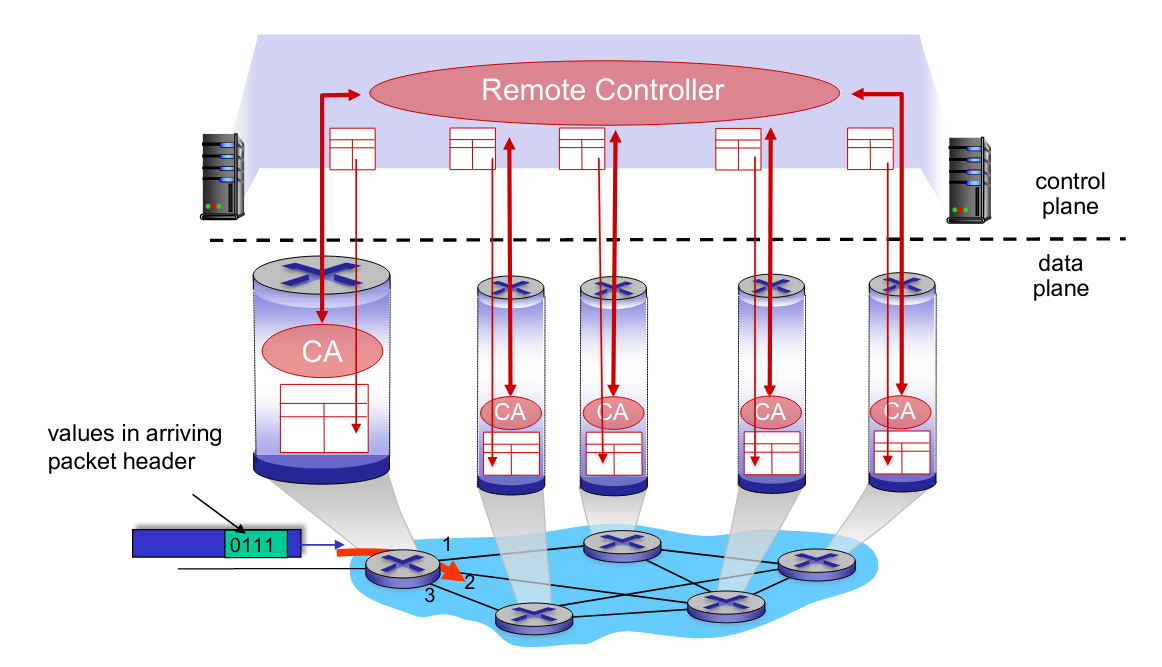
\includegraphics[width=\textwidth - 25pt]{images/Software-Defined-Networking.png}
                \end{center}
    \end{itemize}

    \subsection*{Network Service Models}
    \begin{itemize}
        \item Internet service models:
        \item[] 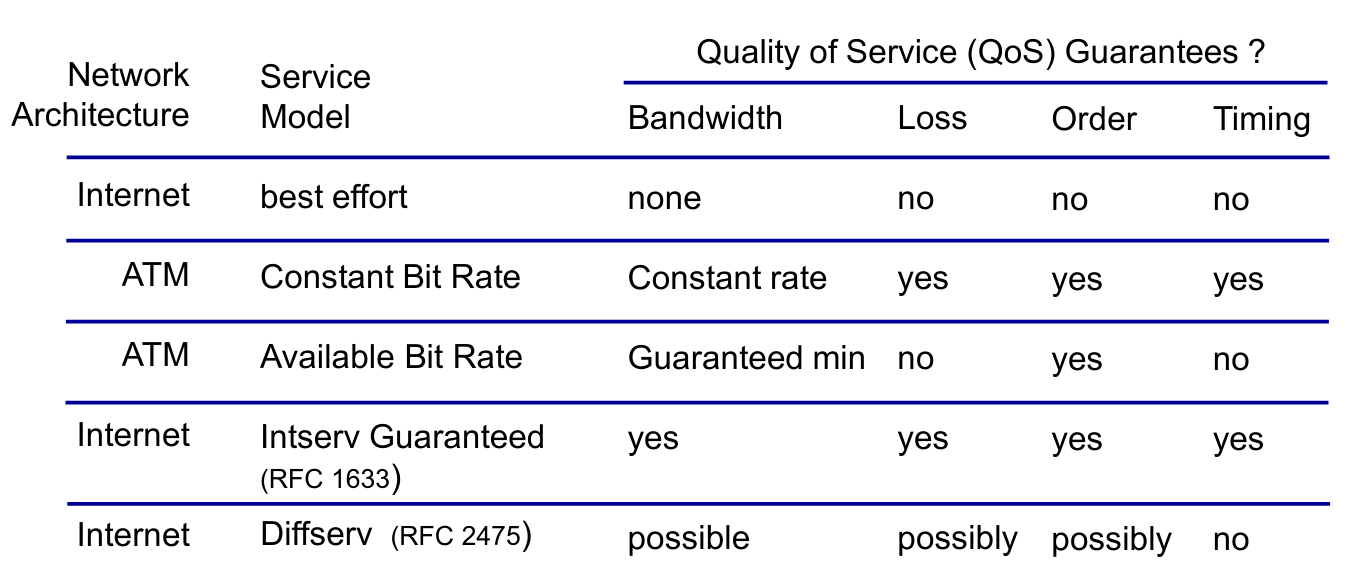
\includegraphics[width=\textwidth - 25pt]{images/Network-Service-Models.png}
        \item Though the \textbf{best effor service model} may not provide any guarantees, it allowed the internet to be widely deployed, and adopted. 
    \end{itemize}

\section*{\centering{Router Architecture Overview}}

    \subsection*{Routers}
    \begin{itemize}
        \item A \textbf{router} is a \textbf{networking device} that \textbf{forwards} and \textbf{router data packets} between \textbf{networks}.
        \item \textbf{Routers} have \textbf{input ports} and \textbf{output ports}, to \textbf{receive} and \textbf{forward} packets respectively.
        \item[] 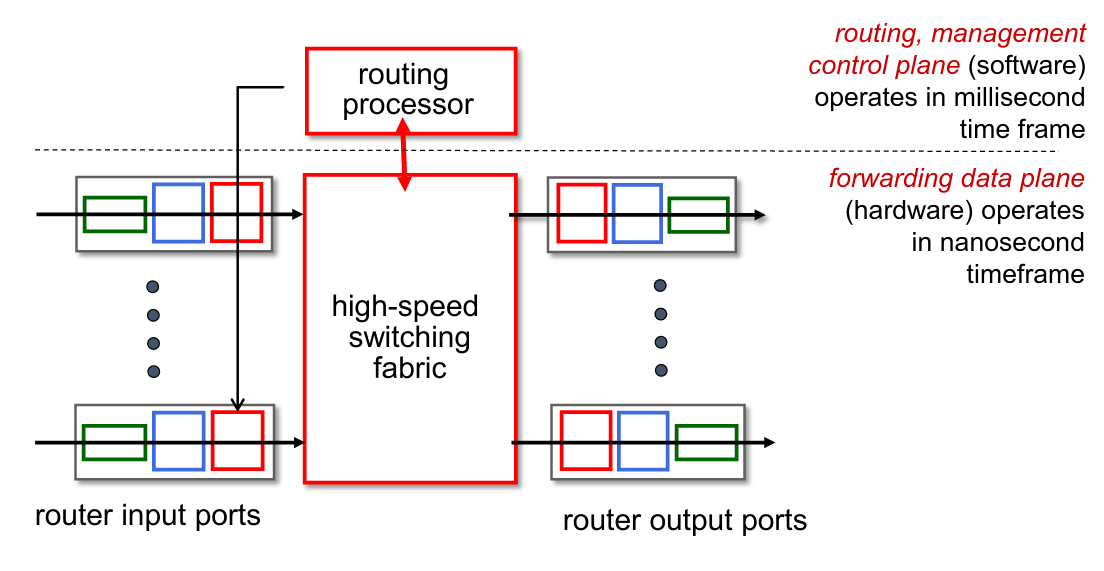
\includegraphics[width=\textwidth - 25pt]{images/Router-Overview.png}
        \begin{itemize}
            \item The green boxes represents the \textbf{physical layer}, the blue boxes represent the \textbf{link layer}, and the red boxes represent the \textbf{network layer}.
            \item The first red box continas a queue of packets that need to be forwarded, and the lookup table, that map headers to ports.
        \end{itemize}
        \item \textbf{Destination-based forwarding} is forwarding based only on the \textbf{destination IP Address} (traditional).
        \item \textbf{Generalized forwarding} is forwarding based on \textbf{any set of header field values}.
        \item The following is an example of a lookup table:
        \item[] 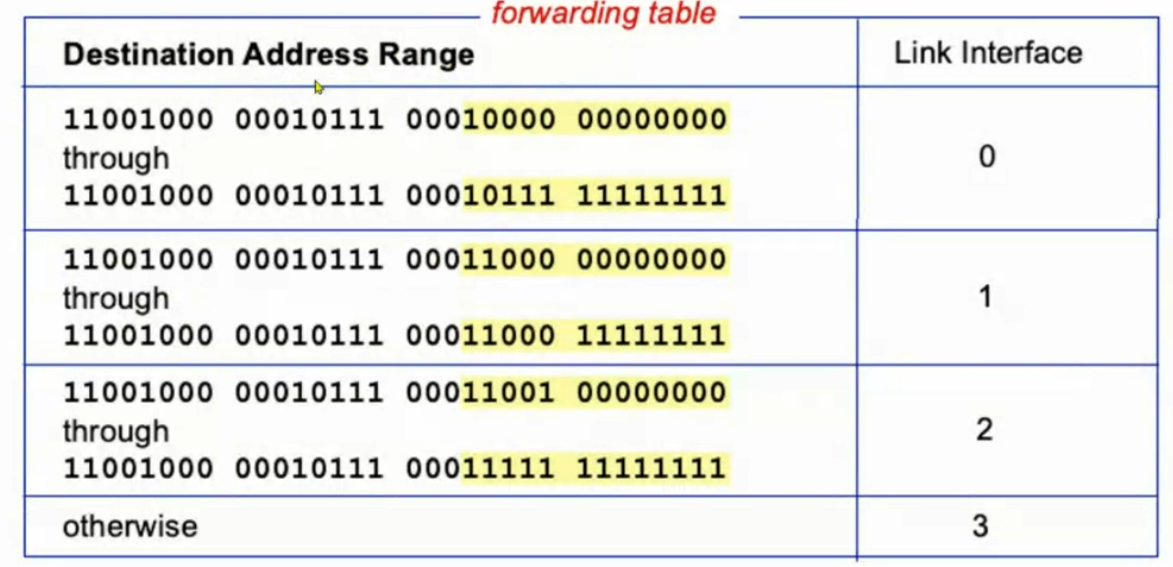
\includegraphics[width=\textwidth - 25pt]{images/Forward-Table.png}
        \begin{itemize}
            \item To determine which interface a an IP address should be mapped to, you see what address range has the longest prefix that matches the IP address of the packet that is being router.
        \end{itemize} 
    \end{itemize}

    \subsection*{Switching Fabrics}
    \begin{itemize}
        \item \textbf{Switching fabrics} are responsible for transfering the \textbf{packet} from the \textbf{input link} to the appropriate \textbf{output link}.
        \item The \textbf{switching rate} is the rate at which \textbf{packets can be trasnferred} from \textbf{inputs} to \textbf{outputs}.
        \item There are \textbf{three main types of switching fabrics}:
        \item[] 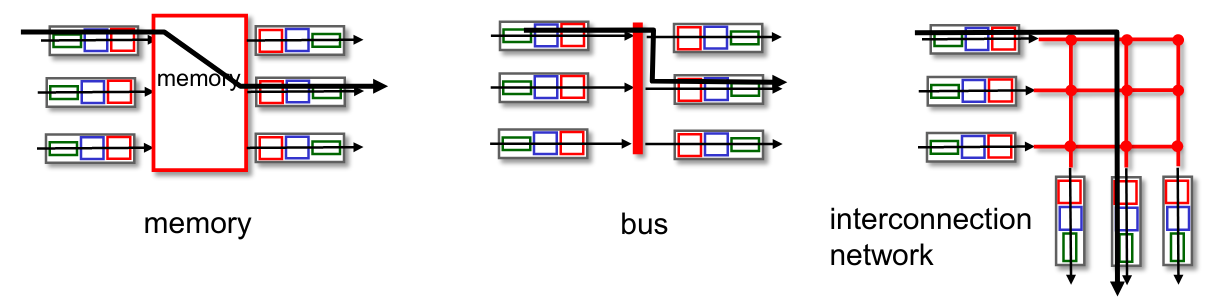
\includegraphics[width=\textwidth - 25pt]{images/Switching-Fabrics.png}
        \item With \textbf{memory switching}, the packets are copied to the \textbf{system's memory}. This limits the switching rate to the \textbf{memories bandwidth}. This type of switching is directly under the control of the \textbf{CPU}.
        \item With \textbf{bus switching}, the packets are delivered from the \textbf{input port's memory}, to the \textbf{output port's memory} directly. The switching speed is limited to the \textbf{speed of the bus} (which is much faster than memory switching). 
        \item With \textbf{interconnnection network switching}, is similar to the bus, except we can \textbf{transfer several packets in parallel}.
        \item We can have \textbf{seveal planes} of \textbf{interconnection network switching} that run in parallel to allow for scaling.
    \end{itemize}

    \subsection*{Input Port Functions}
    \begin{itemize}
        \item There are three functions of an \textbf{input port}:
        \begin{enumerate}
            \item Receives the bits.
            \item Interperates the bits.
            \item Forward the packet to the switching fabric.
        \end{enumerate}
        \item There are two types of \textbf{forwarding} in \textbf{decentralized switching}:
        \begin{enumerate}
            \item \textbf{Destination-based forwarding} | Packets are forwarded based on their destination IP Address.
            \item \textbf{Generalized forwarding} | Packets are forwarded based on any set of header field values.
        \end{enumerate}
        \item If the \textbf{switching fabric} is \textbf{slower} than the \textbf{input ports conbined}, then \textbf{queueing may occur} at the input queues. The queueing may lead to \textbf{delays, and packet loss}.
        \item \textbf{Head-of-Line (HOL) blocking} is when the \textbf{packet} at the \textbf{front of the queue} prevents the \textbf{queue from moving} (due to congestion).
    \end{itemize}

    \subsection*{Output Port Functions}
    \begin{itemize}
        \item There are three functions of an \textbf{output port}:
        \begin{enumerate}
            \item Receive the packet from the switching fabric.
            \item Send the bits.
            \item Send a line termination.
        \end{enumerate}
        \item \textbf{Buffering} is required when \textbf{packets} arrive from the \textbf{switching fabric} faster than the \textbf{link's transmission rate}.
        \item The \textbf{drop policy} is a policy to determine \textbf{which packets to drop} if the \textbf{buffer is full}.
        \item \textbf{Congestion occurs when the output link is slower than the output ports}.
    \end{itemize}

    \subsection*{Determining Buffer Sizes}
    \begin{itemize}
        \item The \textbf{RFC 3439} rule of thumb is that the \textbf{average buffer size} should be equal to $\text{RTT}\times\text{LinkCapacity}$.
        \item There is such a thing as \textbf{too much buffering}; this can increase delays (particularly in home routers).
        \begin{itemize}
            \item \textbf{Long RTTs} lead to \textbf{poor performance} in \textbf{real-time allpcations}.
        \end{itemize}
        \item When the \textbf{buffer is full}, there are two ways to determine the \textbf{packets to drop} when more arrive:
        \begin{enumerate}
            \item \textbf{Tail drop} involves dropping the arriving packets.
            \item \textbf{Priority drop} involves dropping packets on a priority basis.
        \end{enumerate}
        \item 
    \end{itemize}

    \subsection*{Packet Scheduling}
    \begin{itemize}
        \item There are several ways to \textbf{determine the way packets are scheduled}:
        \begin{enumerate}
            \item \textbf{First Come First Serve (FCFS) Scheduling} schedules packets in the \textbf{order they arrive}.
            \item \textbf{Priority Scheduling} schedules packets \textbf{based on their classification} (classifications can be determined by header fields); all higher classified queues get send first.
            \item \textbf{Round Robin (RR) Scheduling} schedules packets \textbf{based on their classification}, but cycles between the different classification queues.
            \item \textbf{Weighted Fair Queueing (WFQ)} is a \textbf{round robin} scheduling algorithm, that assigns each class a weight, and the weight determines the amount of time is spent on each queue.
        \end{enumerate} 
    \end{itemize}

    \section*{\centering{The Internet Protocol}}

    \subsection*{Internet Protocol Datagrams}
    \begin{itemize}
        \item[] \begin{center} \includegraphics*[]{images/Internet-Protocol-Datagram.png} \end{center}
        \item The \textbf{maximum length} of a \textbf{datagram is 65536 bytes}. However the typical size is around \textbf{1500 bytes or less}.
    \end{itemize}

    \subsection*{IP Address}
    \begin{itemize}
        \item An \textbf{IP Address} is a \textbf{32-bit identifier} associate with each \textbf{network host} or \textbf{router interface}.
        \begin{itemize}
            \item An \textbf{interface} is a \textbf{connection} between a \textbf{host/router} and a \textbf{physical link}.
            \item \textbf{Routers} typically have multiple interfaces, and \textbf{hosts} typically have one or two interfaces.
        \end{itemize}
    \end{itemize}

    \section*{\centering{Subnetworks}}

    \subsection*{Subnetworks (Subnets)}
    \begin{itemize}
        \item A \textbf{subnetwork} is a \textbf{local partition} of an \textbf{Internet Protocol network}.
        \item \textbf{Subnets} are typically defined as a group of \textbf{device interfaces} that can \textbf{physically reach each other} without \textbf{passinging through an intervening router}.
        \item \textbf{Devices} in the \textbf{same subnet} have \textbf{common high order bits} in their \textbf{IP Addresses}, and the \textbf{low order bits differ between hosts}.
        \begin{itemize}
            \item For example, the following addresses are an example of a subnet: 1.0.23.1, 1.0.23.5, 1.0.23.10
        \end{itemize}
        \item A \textbf{subnet mask} is a \textbf{32-bit number} created by setting \textbf{host bits to 0}, and \textbf{network bits to 1}. All bits set to 0 can change, and the addresses will still be a part of the subnet.
        \begin{itemize}
            \item There is a short hand for this, you put a slash and then the number of bits that are set to 1 starting from the left. For example /24 = 11111111.11111111.11111111.00000000
            \item You can also express subnet masks as their decimal interpretation: \newline 11111111.11111111.11111111.00000000 = 255.255.255.0
        \end{itemize}
        \item There are \textbf{three main classes} of networks:
        \begin{enumerate}
            \item \textbf{Class A} networks have a subnet mask of \textbf{255.0.0.0}.
            \item \textbf{Class B} networks have a subnet mask of \textbf{255.255.0.0}.
            \item \textbf{Class C} networks have a subnet mask of \textbf{255.255.255.0}.
        \end{enumerate}
        \item There is also a \textbf{Class D and Class E}, but they are reserved for special purposes, and research. They are not available for network hosts.
    \end{itemize}

    \subsection*{Gateways}
    \begin{itemize}
        \item Each \textbf{inteface} on a \textbf{router} has a \textbf{unique IP Address}.
        \item \textbf{Routers} that provide an \textbf{interface} between \textbf{two distinct subnetworks} are known as a \textbf{gateway}.
        \begin{itemize}
            \item Gateways are a router that interfaces multiple subnets, hence why each inteface gets a unique IP Address that must be within the subnet it is interfacing with.
            \item When at least two gateways are directly connected, there is a new subnet between them.
        \end{itemize}
    \end{itemize}

    \subsection*{IP Adressing | CIDR}
    \begin{itemize}
        \item \textbf{Classless InterDomain Routing (CIDR)} (aka supernetting) is a \textbf{method of assigning Internet Protocol (IP) adresses}.
        \item \textbf{CIDR} consists of the following address format: \textbf{a.b.c.d/x} where a, b, c, d are n-bit numbers numbers, and x is the number of bits in the subnet portion of the address.
        \begin{itemize}
            \item An example would be \textbf{200.23.16.0/23}, the first 23 bits identify the subnetwork, and the last 9 bits identify the host within the subnetwork.
        \end{itemize}
        \item There are to ways a \textbf{host} gets an \textbf{IP Address assigned}:
        \begin{enumerate}
            \item \textbf{A Hard-coded address} that is assigned by a sysadmin in a configuration file.
            \item \textbf{The Dynamic Host Configuration Protocol (DHCP)} which allows devices the get IP Adress assignments dynamically from a server.
        \end{enumerate} 
        \item DHCP is particularly useful for devices connecting to routers over \textbf{Wi-Fi}. 
    \end{itemize}
    
    \subsection*{Dynamic Host Configuration Protocol}
    \begin{itemize}
        \item The goal of \textbf{DHCP} is to allow \textbf{hosts} to \textbf{dynamically obtain IP Adresses} from a \textbf{network server} when it "joins" the network.
        \item \textbf{DHCP "leases"} out \textbf{IP Adresses} to devices on the \textbf{network} for a \textbf{specific period of time}. This allows for addresses to be \textbf{reused} if a device leaves the network.
        \item The process is \textbf{seamless} so hosts can easily come and go.
        \item The following is how a device \textbf{typically obtains an IP Address over DHCP}:
        \begin{enumerate}
            \item The \textbf{host} broadcasts a \textbf{DHCP discover} message (only if the host does not know the address of the DHCP server).
            \item The \textbf{DHCP server} responds with a \textbf{DHCP offer} message (only if the host sends a discover message).
            \item The \textbf{host} requests the \textbf{IP Address} that the \textbf{server} offered with a \textbf{DHCP request} message.
            \item The \textbf{DHCP server} sends a \textbf{DHCP ack} message to the \textbf{address} that has been \textbf{leased to the host}.
        \end{enumerate}
        \item Typically, the \textbf{DHCP server} will be \textbf{co-located in the router}, serving all \textbf{subnets} the \textbf{router is attached to}.
        \item When \textbf{DHCP} messages are sent, the \textbf{server} typically uses port \textbf{67}, and the host typically uses port \textbf{68}.
        \item[] \includegraphics*[width=\textwidth - 25pt]{images/DHCP-Request.PNG}
        \item \textbf{DHCP} can return more than just an \textbf{IP Address}, it can also return:
        \begin{enumerate}
            \item The \textbf{address} of the \textbf{first-hop} router for a \textbf{client}.
            \item The \textbf{name} and \textbf{IP} of a \textbf{DNS server}.
            \item The \textbf{network mask} (including network vs host portion of an address).
        \end{enumerate}
    \end{itemize}

    \subsection*{Internet Service Providers}
    \begin{itemize}
        \item The \textbf{Internet Corporation for Assigned Names and Numbers (ICANN)} is responsible for \textbf{assigning IP address blocks} to \textbf{Internet Service Providers (ISPs)}.
        \item The \textbf{ISPs} can then assign them to their clients.
    \end{itemize}

    \subsection*{Network Address Translation (NAT)}
    \begin{itemize}
        \item All \textbf{devices} in a \textbf{local network} share \textbf{one public IPv4 address} as far as the outside world is concerned (the address of the first-hop router).
        \item \textbf{Datagrams} with a \textbf{source} or \textbf{destination} within this network have \textbf{10.0.0.0/24} or \textbf{192.168.0.0/24} as the \textbf{source and destination address} (usually).
        \item All \textbf{datagrams} that are \textbf{leaaving the local network} have the \textbf{same source NAT IP Address}, but different \textbf{source port numbers}.
        \item All \textbf{devices} in the \textbf{local network} have a \textbf{private 32-bit IP Address} that can only be used in the \textbf{local network}.
        \item The advantage that is provided by allowing \textbf{one public IP Address} to map to \textbf{several private IP Addresses} is:
        \begin{enumerate}
            \item The ISP only needs to assigne one address to the customer for all devices on the local network.
            \item You can change the address of hosts in a local network without notifying the outside world.
            \item You can change ISP providers without changing addresses of devices in the local network.
            \item Enhanced security; devices inside the local network are not directly addressable or visible by the outside world, instead they are proxied.
        \end{enumerate}
        \item In 2011, ICANN allocated the last remaining available IPv4 addresses to an ISP, public and private IP Adresses allow us to remain on IPv4 for longer, because the same addresses are reused in several local networks.
    \end{itemize}

    \subsection*{NAT Implementation}
    \begin{itemize}
        \item The NAT router must transparently do the following:
        \begin{enumerate}
            \item \textbf{Outgoing Datagrams} | The source IP and port of every datagram must be replaced by the NAT IP and a new port which identifies the host in the local network. Remote hosts will respond using the new NAT IP address and port. The mapping will be placed in a NAT table.
            \item \textbf{Incoming Datagrams} | The destination IP and port of every datagram must be replaced with the with the original local IP and port, which were previously stored in a NAT table.
        \end{enumerate}
    \end{itemize}

    \subsection*{The NAT Controversy}
    \begin{itemize}
        \item Nat has been controversial:
        \begin{itemize}
            \item \textbf{Routers} should only process \textbf{up to layer 3} (ports are layer 4).
            \item The \textbf{address shortage} should be solved by \textbf{IPv6}, not \textbf{NAT}.
            \item It \textbf{Violates} the \textbf{end-to-end argument} (port \# manipulation).
            \item It doesnt allow \textbf{clients} to \textbf{connect} to \textbf{servers behind NAT}.
        \end{itemize}
        \item Even with all of th controversy, NAT is here to stay. It is extensively used in home and institutional networks, and 4G/5G cellular networks.
    \end{itemize}
    
    \subsection*{Middlebox Functions}
    \begin{itemize}
        \item A \textbf{Middlebox} is an \textbf{intermediary box} that performs \textbf{functions} \textbf{apart from the noraml, standard functions} of an \textbf{IP router} on the \textbf{data path} between a \textbf{source host} and a \textbf{destination host}.
        \item Some exampls of middleboxes are firewalls, NAT, load balancers, CDN cache, etc.
        \item Initially, \textbf{middleboxes were proprietary} hardware solutions.
        \item Over time, things moved towards \textbf{open solutions} with \textbf{programmable local actions} via match+action.
        \item \textbf{Software-Defined Networking (SDN)} allows for \textbf{logically centralized control} and \textbf{configuration managment}, often in the \textbf{"cloud"}.
    \end{itemize}

    \section*{\centering{Internet Protocol version 6 (IPv6)}}
    
    \subsection*{IPv6 Format}
    \begin{itemize}
        \item The \textbf{initial motivation} was the fact that \textbf{IPv4 addresses} would be (at the time they were not completely allocated, they are now) \textbf{completely allocated}.
        \item Unlike IPv4, the IPv6 format does not have \textbf{a checksum, options, or fragmentation}.
        \item A major problem is that not all routers can be upgraded simultaneously.
        \item To allow \textbf{routers} that \textbf{only support IPv4, to handle IPv6 datagrams}, we can use \textbf{tunneling}: The \textbf{IPv6 datagram} is carried as a \textbf{payload} in an \textbf{IPv4 datagram}. This is essentially, a packet within a packet.
        \item Tunneling is used extensively in other contexts such as 4G/5G.
        \item[] \includegraphics*[width=\textwidth - 25pt]{images/IPv6-Format.PNG}
    \end{itemize}
    
\end{document}